\title{Siftables Emulator: Deployment and Usage}
\author{Singularity Software}
\date{\today}

\documentclass[12pt]{article}
\usepackage[a4paper]{geometry}
\usepackage{makeidx}
\usepackage{lscape}
\usepackage{amsmath}
\usepackage{graphicx}
\usepackage[final]{pdfpages}

\geometry{top=1.0in, bottom=1.0in, left=1.0in, right=1.0in} % Sets the margins

\setlength{\parindent}{0pt} % Fixes the paragraph spacing problem

\renewcommand*\arraystretch{1.5}

\begin{document}

\begin{center}
	\LARGE{Siftables Emulator} \\
	\LARGE{\textit{Deployment and Usage}}\\
	\Large{\textit{Singularity Software}} \\
	\vspace{.05in}
	\normalsize{\today} \\
\end{center}

\section{Install the emulator}
Siftables Emulator is a cross-platform Silverlight application. To install it for the first time:
\begin{enumerate}
\item Build the project using the Release configuration in Visual Studio.
\item Open [project root]/Siftables/Bin/Release/SiftablesEmulator.html in a Silverlight-compatible web browser.
\item When the app loads, right click anywhere and choose "Install Siftables Emulator onto this computer..."
\item Follow the install wizard, choosing your preferred shortcut locations.
\item Siftables Emulator should launch automatically. If not, it can be launched from wherever you opted to install shortcuts in the previous step.
\end{enumerate}

\section{Walkthrough: Interact with the emulator}

\section{Program for the emulator}
\subsection{Application Programming Interface}
The Siftables Emulator can be programmed using the official Sifteo API available at http://developer.sifteo.com/. The team believes that our implementation of the API outlined there is complete and is functionally on par with the native Sifteo.dll provided for use with the physical Sifteo cubes. This implementation is a combination of work done by the team specifically for Silverlight and the Siftables project and work done by the Sifteo team. The latter part comes in the form of SifteoExtensions.dll, a partial version of Sifteo.dll decompiled and retargeted to Silverlight with Sifteo's permission.

\subsection{Target the emulator}
To target an application targeted for Sifteo Cubes to run in Siftables Emulator, make the following 2 changes:
\begin{enumerate}
\item Create a new Silverlight Application Project and add your existing project files to it.
\item Add references in that project to [project root]/Siftables/Bin/Release/Sifteo.dll and /SifteoExtensions.dll. Note that those DLLs will only exist if you have already built the Release configuration of the emulator as specified in the Deployment/installation instructions.
\end{enumerate}

\section{Walkthrough: Prepare and run an application}
\begin{enumerate}

\item Create a new project for the application.
\begin{enumerate}
\item Select the Silverlight template group in the left pane, then select Silverlight Application in the center.
\item Give the application a name and a location. We recommend not creating a directory for the solution.
\begin{center}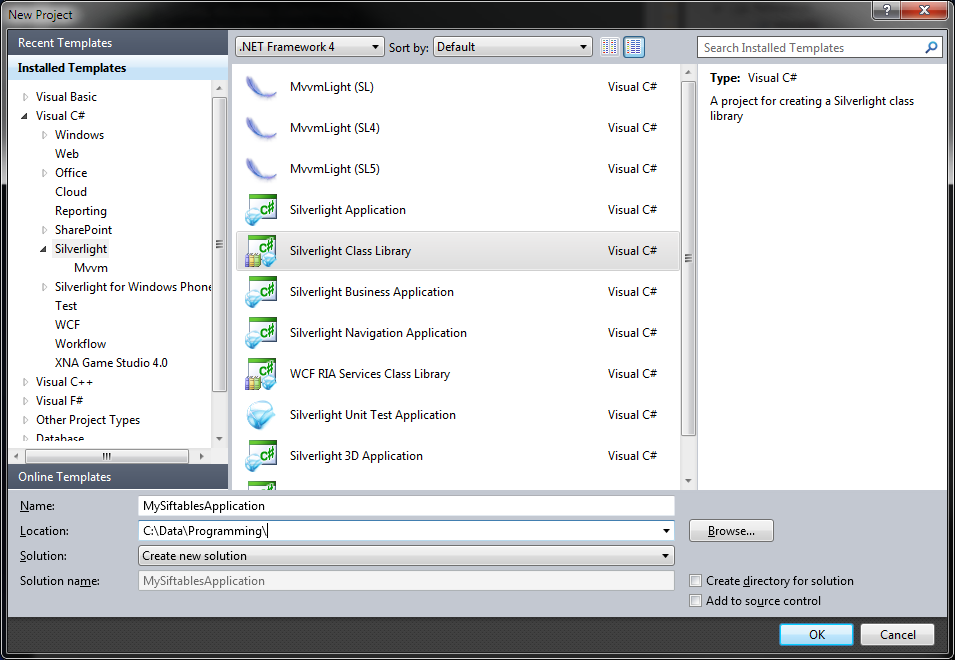
\includegraphics[width=4in]{1-1-NewProjectDialog}\end{center}
\item Ensure that you use Silverlight version 5.
\begin{center}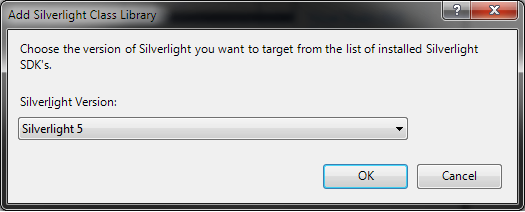
\includegraphics[width=4in]{1-2-NewSilverlightApp}\end{center}
\item Add Sifteo.dll and SifteoExtensions.dll to the project references.
\begin{center}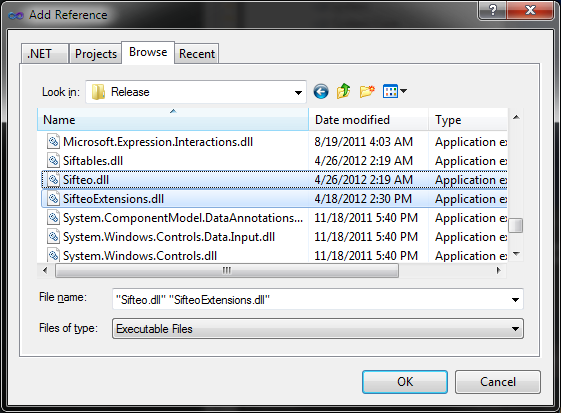
\includegraphics[width=4in]{1-3-AddReferences}\end{center}
\end{enumerate}

\item Build a blank runnable application.
\begin{enumerate}
\item Create a new class.
\item Have it use the Sifteo namespace.
\item Have it extend BaseApp.
\begin{center}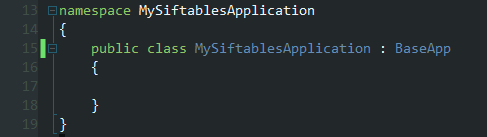
\includegraphics[width=4in]{2-1BlankApp}\end{center}
\item Build the solution. Note the location of the DLL in Output.
\begin{center}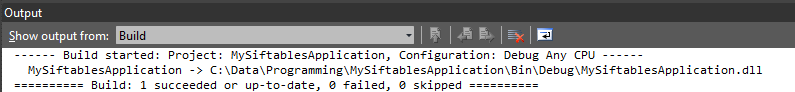
\includegraphics[width=4in]{2-2Output}\end{center}
\end{enumerate}

\item Run the blank application in the emulator.
\begin{enumerate}
\item Launch the emulator.
\item Click "Load A Program".
\item Select the DLL built in the previous step.
\item Click Open.
\begin{center}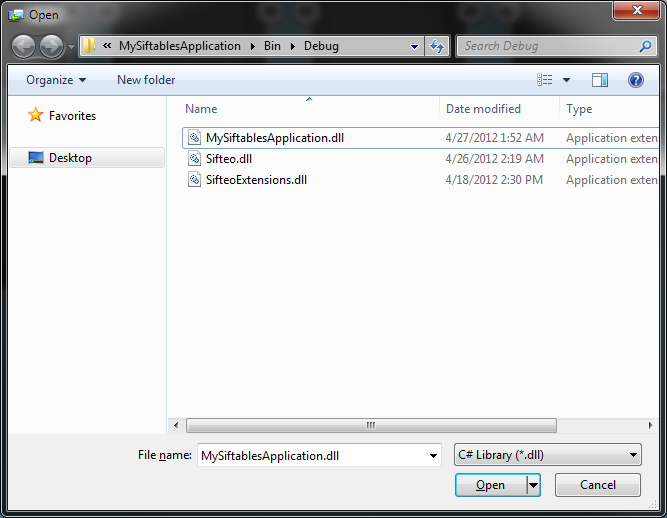
\includegraphics[width=4in]{3-1Open}\end{center}
\end{enumerate}
At this point, you have a fully runnable Siftables application. It doesn't do anything... but that part is up to you!\\

\end{enumerate}

\section{Walkthrough: Respond to cube events}

\end{document}
